\documentclass[12pt]{article}
\usepackage[utf8]{inputenc}
\usepackage{graphicx}
\usepackage{geometry}
\usepackage{tocloft} 
\usepackage[hidelinks]{hyperref}  
\renewcommand{\cftsecleader}{\cftdotfill{\cftdotsep}}
\usepackage{apacite}
\bibliographystyle{apacite}


\geometry{margin=1in}

\begin{document}
\thispagestyle{empty}

\begin{center}
\begin{figure}
  \centering
  
  
\includegraphics[height=3.5cm]{logo-tec.png} 
\end{figure}

\vspace{0.5cm}

\small
\textbf{COSTA RICA INSTITUTE OF TECHNOLOGY\\
    ALAJUELA ACADEMIC CENTER\\
    COMPUTER ENGINEERING DEPARTMENT}

\vfill
\huge
\textbf{Project 0: The Narrow Bridge Simulation} \\
\vspace{0.5cm}
\large
\textit{An Implementation of Concurrency and Process Synchronization}

\vfill
\small 
\textbf{IC-6600 Principles of Operating Systems} \\
I Semester, 2026

\vfill
\small
By:\\
\large
\textbf{Angie Esquivel López} \\ 
\textbf{Alejandro Quesada Calderón} \\ 
\textbf{Esteban Espinoza Solano} \\ 


\vfill

\normalsize
\textbf{Prof. Eddy Ramírez Jiménez}

\vfill
\small
Alajuela, March 19, 2026
\end{center}

\newpage
\vfill
\tableofcontents


\newpage
\section{Introduction}

The development of modern computing relies on concurrent execution and efficient resource management. This project aims to provide a solid understanding of both the basic theory and practice of these systems. The primary purpose of this project is to build with basic thread management and concurrency, and with that solving classic operating system problems. This implementation exposes the developer to an environment with multiple processes that must be scheduled by the operating system.

To achieve this, the project simulates the narrow bridge problem. The simulation models a city bridge connecting an East and West sector. Because the bridge is obsolete and only wide enough for one car, it only allows unidirectional traffic at any given time. This physical constraint demands careful administration to maximize the utilization of the bridge, minimize waiting times, and ensure fair allocation of the resource.

The solution is programmed entirely in C on a Linux environment. It utilizes the Pthreads library to handle the execution threads. Because Pthreads is based on the POSIX standard, it serves as a highly useful tool for utilizing system services through system calls. Every entity in the simulation, such as vehicles, traffic lights, and police officers, is represented by an individual thread. Consequently, the project requires strict administration of process synchronization to maintain order and actively prevent deadlocks.
\newpage

\section{Theoretical Framework}
This section outlines the foundational concepts underpinning the concurrent simulation, establishing the theoretical basis for managing shared resources in a multiprogrammed environment.

\subsection{Operating Systems and Interfaces}
The foundation of any hardware-level simulation is the operating system itself. An operating system is software that manages a computer’s hardware. It also provides a basis for application programs and acts as an intermediary between the computer user and the computer hardware \cite[Chap.~1, p.~3]{silberschatz_os}.

To interact with this underlying system, programs must use specific interfaces. System calls provide the essential interface between a running user program and the operating system kernel. They allow processes to request privileged operations safely, such as creating new threads, managing hardware resources, or performing I/O operations \cite[Chap.~2, p.~62]{silberschatz_os}.

\begin{figure}[h!]
  \centering
  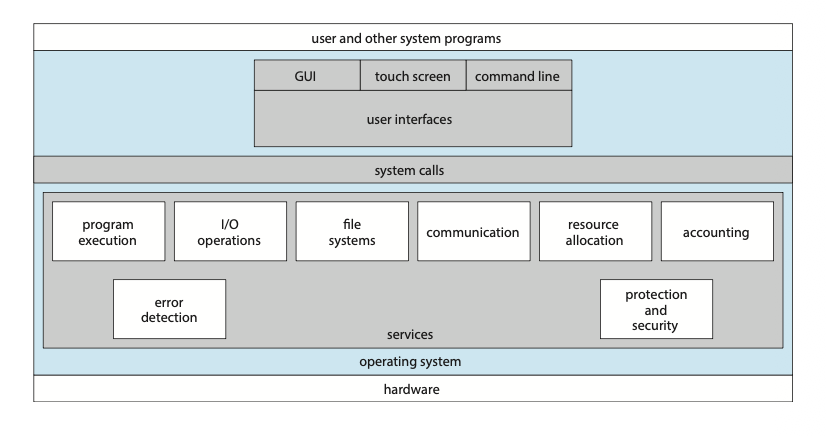
\includegraphics[height=5.5cm]{SystemCall.png}
\end{figure}

\subsection{Concurrency and Threads}
When multiple operations are initiated via system calls, the system must handle them simultaneously. We use this conceptual term to refer to a host of problems that arise, and must be addressed, when working on many things at once (i.e., concurrently) in the same program. The problems of concurrency arose first within the operating system itself; the OS is juggling many things at once, first running one process, then another, and so forth \cite[Chap.~2, p.~6]{three_easy}.

To achieve this concurrency efficiently, modern operating systems utilize threads. A thread is a basic unit of CPU utilization; it comprises a thread ID, a program counter, a register set, and a stack. It shares with other threads belonging to the same process its code section, data section, and other operating-system resources, such as open files and signals. A traditional (or heavyweight) process has a single thread of control. If a process has multiple threads of control, it can perform more than one task at a time \cite[Chap.~4, p.~160]{silberschatz_os}.



\subsection{CPU Scheduling}
Because concurrent execution relies on sharing a limited number of processors, dynamic administration becomes critical. A process migrates among the ready queue and various wait queues throughout its lifetime. The role of the CPU scheduler is to select from among the processes that are in the ready queue and allocate a CPU core to one of them. The CPU scheduler must select a new process for the CPU frequently. An I/O-bound process may execute for only a few milliseconds before waiting for an I/O request. Although a CPU-bound process will require a CPU core for longer durations, the scheduler is unlikely to grant the core to a process for an extended period. Instead, it is likely designed to forcibly remove the CPU from a process and schedule another process to run \cite[Chap.~3, p.~113]{silberschatz_os}.

\subsection{Process Synchronization and Deadlocks}
When multiple threads execute concurrently and share resources, such as a narrow bridge, data integrity must be maintained. This requires process synchronization. A critical section is a piece of code that accesses a shared resource, usually a variable or data structure. To avoid race conditions, we need to ensure that only one thread can execute within the critical section at a time. This is known as mutual exclusion \cite[Chap.~28, p.~3]{three_easy}.



Improper scheduling and resource allocation among concurrent processes can lead to catastrophic system states. For many applications, a process needs exclusive access to not one resource, but several. Suppose, for example, two processes each want to scan an object with a 3D scanner and then print the front, top, and side view of the object on a printer. Process A requests permission to use the 3D scanner and is granted it. Process B is programmed differently and requests the printer first and is also granted it. Now A asks for the printer, but the request is suspended until B releases it. Unfortunately, instead of releasing the printer, B asks for the 3D scanner. At this point both processes are blocked and will remain so forever. This situation is called a \textbf{deadlock} \cite[Chap.~6, p.~437]{modernOS}.

\section{Solution Description}
\section{Conclusions}
\section{Experience Description}
\section{Personal Key Takeaways}


\bibliographystyle{apa}
\bibliography{source}
\end{document}